\section{Experiments}

To assess the efficacy of our proposed technique, we have conduct experiments to address the following research question: \textit{Does combining latent and meta path-based topological features improve relationship prediction accuracy in DHINs?}

%We will first introduce the experiment setting, then show the results and analysis on the two types of datasets respectively.

\subsection{Experiment Setup}

%\subsubsection{Dataset.} We conduct our experiments on two real-world datasets, whose statistics are summarized in Table 2. These databases have different characteristics and evolution behaviour. We also consider different type of target relationship as discussed in subsection \ref{targetRelashipSection}.
\subsubsection{Dataset.} We conduct our experiments on two real-world datasets that have different characteristics and evolution behaviour. 


\begin{itemize}
    \item \textit{Publications dataset:} The \textit{aminer} citation dataset\footnote{\url{https://aminer.org/citation}} V8 (2016-07-14) is extracted from DBLP, ACM, and other sources. It contains 3,272,991 papers and 8,466,859 citation relationships for 1,752,443 authors, who published in 10,436 venues, from 1936 to 2016. 78,635 authors had no co-author (about 4\%). 
    
    179,607 authors had no co-author in 1996-2016. 
    78,635 authors had no co-author (about 4\%). 
    ------------
    100,972 (those who published in 1930-1996)?
    
    1,752,443 (total) - 100,972 = 1,651,471 (those who published in 1996-2016)?
    
    1,544,408 authors had no co-author in 1930-1996
    78,635 authors had no co-author (about 4\%). 
    ------------
    1,465,773 (those who published in 1996-2016)?

    1,752,443 (total) -1,465,773 = 300,000 (those who published in between)?
    
%    1,752,443 author_papervenuelist_map
%    2,811,533 paper_authorslist_map
%    10,163 venue_paperauthorslist_map
    
    Each paper is associated with abstract, authors, year, venue, and title. \amin{We consider only those papers published since 1996, which includes 2,935,679 papers and Y authors.} Authors in \cite{sun2011ASONAM} used a similar dataset but considered only authors with more than 5 publications. We generate two datasets: one that contains all publications, and one that considers authors with at least 5 papers. We consider $k=3, 5, and 10$ different time intervals for the dynamic analysis. In our evaluation, we execute the learned model on the last interval to measure the prediction accuracy.
    
    \item \textit{Movies dataset:} The RecSys HetRec 2011 movie data set \cite{Cantador:RecSys2011} is an extension of MovieLens10M dataset, published by GroupLeans research group \footnote{\url{http://www.grouplens.org}} that links the movies of MovieLens dataset with their corresponding web pages at Internet Movie Database (IMDB\footnote{\url{http://www.imdb.com}}) and Rotten Tomatoes\footnote{\url{http://www.rottentomatoes.com}} movie review systems. It contains information of 2,113 users, 10,197 movies, 20 movie genres (avg. 2.04 genres per movie), 4,060 directors, 95,321 actors (avg. 22.78 actors per movie), 72 countries, 855,598 ratings (avg. 404.92 ratings per user, and avg. 84.64 ratings per movie), and 13,222 tags (avg. 22.69 tas per user, avg. 8.12 tas per movie).

\end{itemize}


Movies once release, users can rate them but a paper is published once and new co-authorship is made only at that time... In Publications dataset co-authorship connections are new in Movies dataset new connections to an existing movie. This is a common problem with all rating datasets.

%Datasets of different sizes.
We also conduct our experiments on two variations of the DBLP, one with min 5paper as in ... and one with all.


%\begin{table}[]
%\centering
%\caption{Comparison of the two networks.}
%\scriptsize
%\begin{tabular}{lllll}
%Network      & Size & Target MP & MP length & \#Training \\
%Publications &      &           &           &            \\
%Movies       &      &           &           &            \\
%             &      &           &           &           
%\end{tabular}
%\end{table}

\subsubsection{Experiment Settings.} 
- Parameters

- Baseline methods .Considering the effect of time-wise data decomposition. What if we shorten timespans of each $G_t$? The extreme is having only one graph or having it for each year. Can we find a trade-off?

\begin{itemize}
    \item  Heterogeneous non-temporal (PathCount, PathSim, NormalPathCount, RandomWalk, SymmetricRandomWalk)
    \item  Homogeneous non-temporal (Katz, Jaccard)
    \item  Homogeneous temporal (BCGD)
\end{itemize}

- Meta paths and target relationships. Figure \ref{Fig:expSchema} depicts network schemas for the two datasets. Note that we consider a simplified version and ignore nodes such as topic fro papers or tag for movies.

We consider .... based on the work in ... we con

%conducted Wald test in a case study and found that the $p$-value for the feature associated with each meta path and their significance level. From the results, we can see that the 

Table \ref{table_publications} shows meta paths between authors under length 4 for the publications dataset.


Authors in \cite{sun2011ASONAM} conducted a case study on a similar DBLP dataset and found that shared co-authors, shared venues, shared topics and co-cited papers for two authors play very significant roles in determining their future collaborations. Similarly we consider meta paths including \textit{A--P--A} (target meta path), \textit{A--P--V--P--A}, \textit{A--P--A--P--A}, and \textit{A--P--P--P--A}.

We consider different type of target relationship.


\begin{figure}[t]
\centering
\subfigure[Publications Network]{
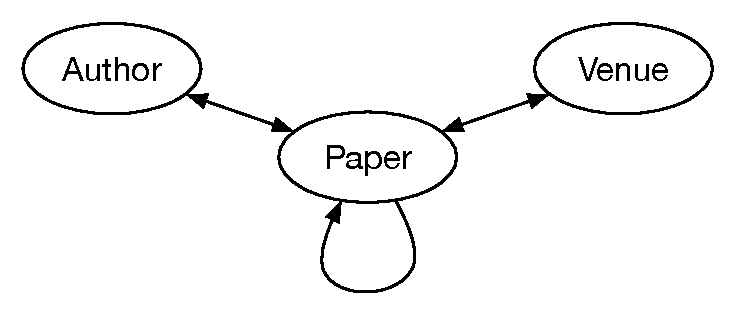
\includegraphics[trim = 0mm 0mm 0mm 0mm,width=0.45\hsize]{figs/publicationsSchema.pdf}
 \label{Fig:DBLP}
}
\subfigure[Movies Network]{
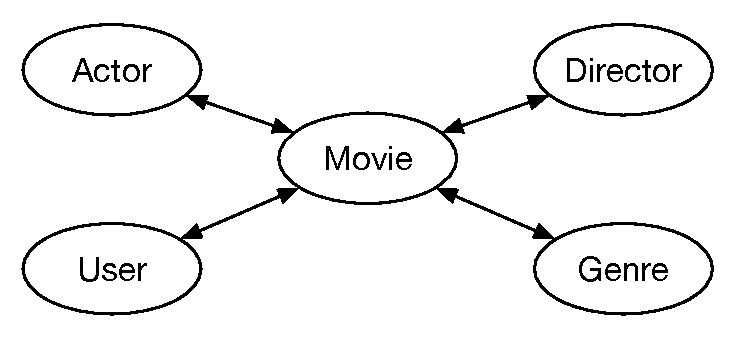
\includegraphics[trim = 0mm 0mm 0mm 0mm,width=0.45\hsize]{figs/moviesSchema.pdf}
 \label{Fig:IMDB}
}
\caption{The simplified network schema used for our experiments.} \label{Fig:expSchema}
\end{figure}


Similarly we only calculated the PC for these meta paths. Note that the goal of our paper is not to select the best features but to show the strength of using...



\begin{table}[h]
\centering
\caption{Publications dataset meta paths (\textit{A} = author, \textit{P} = paper, \textit{A} = venue).}
\label{table_publications}\scriptsize
\begin{tabular}{|c|l|} \hline
\textbf{Meta path} & \textbf{Meaning} \\ \hline

\textit{A--P--A} & [\textit{The target relation}] Authors are coauthors \\ \hline
\textit{A--P--V--P--A} & Authors publish in the same venue \\ \hline
\textit{A--P--A--P--A} & Authors have the same co-author \\ \hline
\textit{A--P--P--P--A} & Authors cite the same papers \\ \hline

\end{tabular}


\end{table}

Unlike the \textit{A--P--A} target relation for the publication dataset for which both ends of the relation is of the same kind, we consider \textit{U--M} as the target meta path for the movie dataset to show the effectiveness of our proposed methods in predicting such relationships.
\amin{The issue with matrix factorization is that originally $G_{n*n}$ is for homogenous network with the same type of nodes. In our case $ZZ^T$ vs. $VU^T$ }

\begin{table}[h]
\centering
\caption{Movies dataset meta paths (\textit{U} = user, \textit{M} = movie, \textit{A} = actor,\textit{D} = director, \textit{G} =g enre).}
\label{table_movies}\scriptsize
\begin{tabular}{|c|l|} \hline
\textbf{Meta path} & \textbf{Meaning} \\ \hline
\textit{U--M} & [\textit{The target relation}] A user watches a movie \\ \hline

\textit{U--M--A--M} & A user watches a movie with the same actor \\ \hline
\textit{U--M--D--M} & A user watches a movie with the same director \\ \hline
\textit{U--M--G--M} & A user watches a movie of the same genre \\ \hline
\textit{U--M--U--M} & A user watches a movie that another user  \\ \hline

\end{tabular}
\end{table}




\subsubsection{Evaluation Metrics.} To asses the link prediction accuracy, we use Area Under Curves (both Receiver Operating Characteristic (ROC) and Precision-Recall (PR) curves), termed as AUCROC and AUCPR \cite{davis2006relationship}. Also in order to decide which classifier has a lower error rate, we perform McNemar's test that assess the significance of the difference between two correlated proportions.


Hi, I have seen various studies use McNemar's test to statistically test the accuracy of several classifications. 

McNemar's Test to compare the predictive accuracy of two models. McNemar's test is based on a 2 times 2 contigency table of the two model's predictions.


fMc Nemar?s test [12, 13] is a variant of c2 test and is a non-parametric test used to
analyse matched pairs of data. According to Mc Nemar?s test, two algorithms can
have 4 possible outcomes arranged in a 2�2 contingency table [14] as shown in
Table 3.

Using this criterion, the z scores are calculated usingMc Nemar?s test for the five
classification algorithms. All the algorithms were used with their default parameters
as parameter tuning may favor one algorithm to produce better results.
The null hypothesis (H0) for this experimental design suggests that different classifiers
perform similarly whereas the alternative hypothesis (H1) claims otherwise
suggesting that at least one of the classifiers performs differently as shown in Equation
2.


In order to decide which classifier performed better, Ns f and Nf s values for two
classifiers are examined. For example, classifier A is said to perform better than
classifier B if Ns f is larger than Nf s according to Table 3.



\subsection{Results and Findings}

\amin{One reason that \textit{A--P--V--P--A} is better with intervals is that one may publish in KDD but there are so many publishing there....}


\subsection{Discussion}

%Increasing accuracy.... We do not claim that the linear combination is the best ... After $p$-value analysis some latent features might be correlated with meta paths. Removing may increase the accuracy or we can remove those with lower $p$-value. This needs careful analysis as it might be dependent to number of intervals or the size of latent feature.


Our proposed technique can also be used in other applications. For example link recommendation 


predicting missing edges in graphs.

Vertex Recommendation similar to \cite{ou2016asymmetric} 


In this work we modelled the predicted graph $ \hat{G}_\tau(i,j)$ as a combination of meta path features and latent features $\Phi(z_{i}^Tz_{j} + f_D(z_{i,j};w))$. As explained in \cite{menon2011link}, one may also augment the model by incorporating some information regarding node affinities using implicit/explicit attributes and define node features $x_i$, which makes the model $\hat{G}_\tau(i,j) = \Phi(z_{i}^Tz_{j} + f_D(z_{i,j};w)$

As shown in \cite{menon2011link} and \cite{Zhu2016}, latent features are more predictive of linking behaviour compared to unsupervised scoring techniques such as Katz, PrefferentailAttachemnet, and Adamic.

Experiments in \cite{menon2011link} shows combining the latent structure and side-information increases the prediction accuracy.


\amin{TODO}
Connection to link privacy research such as \cite{amin:wwwj}

From: Target Defense Against Link-Prediction-Based Attacks via Evolutionary Perturbations

Fard et al. [24] assumed that all links in a network are sensitive, and they proposed to apply subgraph-wise perturbations onto a directed network, which randomize the destination of a link within some subnetworks thereby limiting the link disclosure. Furthermore, they proposed neighborhood randomization to probabilistically randomize the destination of a link within a local neighborhood on a network [25]. It should be noted that both subnetwork-wise perturbation and neighborhood randomization perturb every link in the network based on a certain probability.

As discussed above, link prediction can be applied to predict the potential relationship between two individuals. From another perspective, it may also increase the risk of link disclosure. Even if the data owner removes sensitive links from the published network dataset, it may still be disclosed by link prediction and consequently lead to privacy breach. Michael et al. [26] presented a link reconstruction attack, which is a method that attacker can use link prediction to infer a user?s connections to others with high accuracy, but they did not mention how to defend the so-called link-reconstruction attack. Naturally, one can consider finding a way to prevent the link-prediction attack. Since link-reconstruction attack or link-prediction-based attack aims to find out some real but unobservable links, the defense of link-prediction-based attacks is also target-directed, which means that one has to preserve the targeted links from being predicted. In the literature, most existing approaches on link prediction are based on the similarity between pairwise nodes under the assumption that the more similar a pair of nodes are, the more likely a link exists between them.

In general, since many link prediction algorithms are designed based on network structures, a data owner can add perturbations into the original
network to reduce the risk of targeted-link disclosure due to link-prediction-based attacks


From: SmartWalk: Enhancing Social Network Security via Adaptive Random Walks

Extensive research has been carried out to protect the privacy of trust relationships between any pair of users (link privacy) [19, 20, 50, 54, 33, 27]. The challenge of preserving link privacy lies in causing no significant losses on the utility of applications that leverage the social trust relationships. Specifically, link privacy is preserved by adding extra noise to the local structure of a social network. At the same time, global structural characteristics are maintained to ensure
that the utility of the social network is not severely reduced. This can be implemented by replacing a real link between two users with a fake link generated by a random walk[33]. Link privacy/utility trade-off. Mittal et al. in [33] considered that the length of random walks for all nodes has a fixed value. As the length increases (more noise), the
perturbed social graph converges to a random graph and its utility declines drastically. Our key insight is that instead of adding identical amount of noise to all users, perturbation can be unevenly distributed according to the local mixing time such that privacy can be protected with less perturbation on average. In other words, we can perform nodeadaptive random walks rather than random walks with a fixed length for every user when generating fake links.
[33] P. Mittal, C. Papamanthou, and D. Song. Preserving link privacy in social network based systems. In NDSS, 2013



% visualize the network embeddings and features with t-SNE and use KL divergence to measure the performance

